To build a classifier to recognize different shapes of hands, we used a \textit{mlpy} Machine Learning library for python. This library provides a variety of ML algorithms. The one used for this project is linear support vector machine trained over 5 principle components of the input data.
\subsection*{Principle Component Analysis}
Input vector consists of 12 features of every image sequence. It is believed to be more than what is required to actually represent the data, therefore we performed PCA analysis on the dataset to find best set of components. In figure \ref{fig:pca} we can see that only first 5 contribute to most variation in the dataset. Using the top 5 components we project the dataset into lower 5 dimension manifold.\\

\begin{figure}[htp]
\begin{center}
\leavevmode
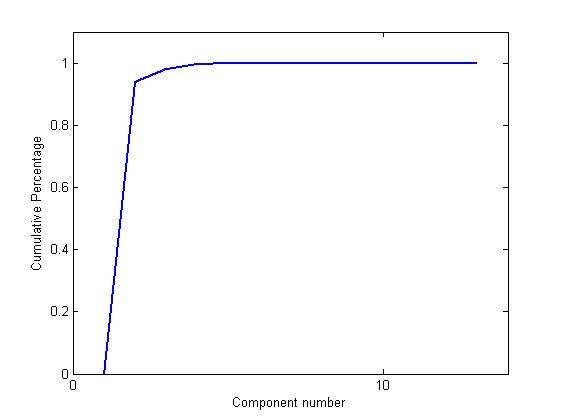
\includegraphics[width=0.6\textwidth] {pca.jpg}
\end{center}
\caption{Cumulative Percentage PCs}
\label{fig:pca}
\end{figure}

\textit{mlpy} library provides a simple API to perform PCA.
\subsection*{SVM}
After obtaining the projected data into 5 PCs we preform linear SVM on the obtained dataset. the algorithm is an implementation of \textit{multi-class support vector classification by Crammer and Singer}. This algorithm is available in mlpy library.
For this section we tested a two different algorithms starting with Logistic Regression. The results for both Linear Logistic Regression and Multi-class SVM are presented in results section.
\subsection*{Cross Validation}
In order to report correct performance measures for our classifier we utilized Leave-one-out Cross-Validation. The algorithm at each step leaves one data out and performs training on the remaining data. Using the trained classifier test instance is checked.

Summary of the classification module is presented in table \ref{tbl:classification}.
\begin{table}
\begin{tabular}{|c|c|}
\hline 
Preprocessing: & Principal Component Analysis with 5 Compenents \\ 
\hline 
Training Algorithm & Multi-class SVM \\ 
\hline 
Performance Measure & Leave-One-Out Cross-Validation \\ 
\hline 

\end{tabular} 
\caption{Summary of Classification Module parameters and algorithms}
\label{tbl:classification}
\end{table}